\documentclass[11pt, oneside]{article}     % use "amsart" instead of "article" for AMSLaTeX format
\usepackage{amsmath}                    % See geometry.pdf to learn the layout options. There are lots.
\usepackage{amsthm}                   % See geometry.pdf to learn the layout options. There are lots.
\usepackage{amssymb}                    % See geometry.pdf to learn the layout options. There are lots.
                % TeX will automatically convert eps --> pdf in pdflatex    
\usepackage{authblk}
\usepackage[utf8]{inputenc}
\usepackage{graphicx}
\usepackage[english,bulgarian]{babel}
\usepackage[T2A]{fontenc}


\newtheorem{mydef}{Дефиниция}[section]
\newtheorem{example}{Пример}[section]
\newtheorem{lem}{Лема}[section]
\newtheorem{thm}{Твърдение}[section]


\title{Рекурсивна публикация \\
(публикация за публикации)}
\author{Калин Георгиев\\ 
\textit{kalin@fmi.uni-sofia.bg}\\
\emph{Факултет по математика и информатика}\\\emph{Софийски университет}}
%\date{}              % Activate to display a given date or no date

\DeclareMathOperator{\restrict}{\upharpoonright}




\begin{document}
\maketitle

\begin{abstract}
 Тази публикация описва един подход за създаване на научни и научно-технически публикации. Разгледани са препоръчителна структура на научните публикации и са дадени насоки, примери и препоръки за подготовката на текста на публикацията. Споменати са някои добри и някои лоши практики при писането на научни публикации.
\end{abstract}

\section{Въведение}
\begin{figure}[htbp]
  \centering
  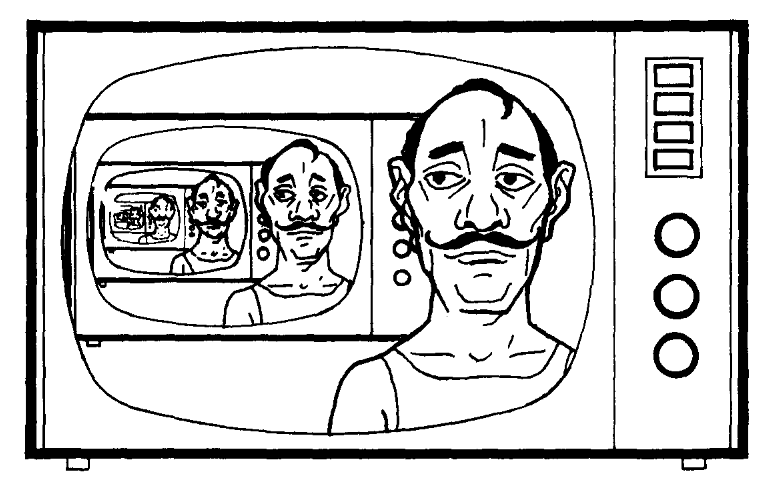
\includegraphics[width=6.5cm]{images/wirth}
  \caption[Да погледнем към себе си \cite{wirth}]
   {Публикация за публикации \cite{wirth}}
  \label{fig:wirth}
\end{figure}


\subsection* {Предметна област: Научна комуникация}

В академичния свят е утвърден развит механизъм, по който учените, инженерите и въобще изследователите споделят с академичната общност своите открития, разсъждения или наблюдения относно въпроси, проблеми и феномени, които представляват интерес за общността или поне за някаква част от нея. Основен роля в научния комуникационен процес играе публикацията или още - статията. Публикациите съдържат текст, фигури, данни, диаграми и пр., чиято цел е да информират общността относно проблема, над който е работил авторът, да предоставят описание на наблюдението, което е извършил, или пък да опишат намерено решение или поне опит за намиране на решение на въпросния проблем. Публикациите достигат до аудиторията си най-често чрез научни и технически списания, както и чрез сборници от конференции.

Академичната общност е твърде нехомогенна, особено що се отнася до разнообразието на научни и технически дисциплини - от двигатели с вътрешно горене до антично изкуство и философия на духа. Макар тази  нехомогенност да затруднява правенето на твърде големи обобщения относно всякакви практики, възприети от отделните дисциплини, при съставянето на научни публикации се наблюдават редица паралели,  общи черти и стандарти. Нещо повече, стилът и последователността на академичните публикации са своеобразна матрица, по която често се съставят публикации извън академичния свят - популярни статии, технически съобщения и пр. Следователно, познаването поне до известна степен на академичния стандарт за писане на текст би могло да бъде полезен инструмент в ръцете на всеки пишещ относно решения и разсъждения по проблеми, касаещи аудиторията му. 

Въпреки шансовете да се намери известна универсалност в правилата за писане на публикации, тази публикация се ограничава до природните и инженерните науки с цел яснота и по-голяма евентуална полезност, като някои твърдения в нея вероятно са невалидни за други дисциплини и направления.
 
\subsection*{Предмет и цел на статията}

Предметът на разглеждане на тази публикация са академичните публикации и по-точно правилата при съставянето им, свързани с органзиацията на текста и въпросите, на които се отговаря в тях. Разгледани са основните характеристики на научната публикация - от какви части е съставена тя, на какви въпроси отговарят тези нейни части и по какъв начин. Целта на статията да даде начални насоки на студентите, на които предстои подготовкака на доклад по курсов проект, статия и изобщо учебно-научен текст.

Относно това доколко изложената тук информация и дадените препоръки представляват утвърден академичен стандарт, то авторът не се ангажира с оценка на този въпрос. Изложената препоръчителна структура следва насоките на известното списание Nature \cite{nature}. Бърз поглед над произволни публикации обаче издава, че тази структура не се спазва точно от почти никоя реална публикация. Следователно, описаните тук структура и препоръки за съставянето на текста би следвало да се разглеждат като обща рамка, която да бъде свободно адаптирана към особеностите на конкретното изследване, списанието, в което се публикува и пр.

\section{Методи и материали}
\subsection*{Използвани инструменти}
Основният инструмент, използван за написването на тази публикация, е пакетът за компютърна типография \LaTeX \cite{latex}. Пакетът е базиран на формален език за описание на документи, чрез който авторите въвеждат съдържанието на публикациите и използват команди, управляващи изгледа му чрез редактор на обикновен текст (plain text).

 Следва пример с кода на \LaTeX, дефиниращ част от тази секция:
\fbox{
  \parbox{\textwidth}{
    \texttt{\textbackslash section \{Методи и материали\} \\
\textbackslash subsection*\{Използвани инструменти\} \\
Основният инструмент, използван за написването на тази публикация, е пакетът за компютърна типография \textbackslash LaTeX \textbackslash cite\{latex\}.}
    
  }
}


 Така съставеният ``изходен код'' на публикацията се компилира от системата на \LaTeX, резултатът от което е PDF документ. Пакетът позволява ``висш пилотаж'' с типографията на документите, но изисква време и усилия за запознаването с езика и особеностите на системата. \LaTeX се ползва най-често в природонаучните дисциплини поради развитите и удобни инструменти за въвеждане и редактиране на математически и технически текст и поради възможността технически запознатите потребители да манипулират директно изходния код на документа, вместо да са принудени да боравят с усложнени и тромави потребителски интерфейси, каквито се наблюдават при съвременните системи за текстообработка.

Системата за текстообработка Microsoft Word е друг широко използван инструмент за писане на академичен текст. Продължителната еволюция на продукта и внушителното многообразие от възможности, достъпни чрез графичен потребителски интерфейс, често го правят предпочитания избор.

Почти всички конференции и научни списания дефинират строги изискваният относно визуалните характеристики на публикациите - големина на полетата, междуредие, шрифт и пр. Както \LaTeX, така и Word предлагат удобни инструменти за дефиниране на шаблони, с чиято помощ авторите могат да спазят изискванията за формат на публикациите почти автоматично.

За написването на тази публикация са използвани също автоматични инструменти за проверка на правописа на думите в текста (spell checkers). Каква гаранция дават те за липса на грешки в настоящия текст авторът няма да коментира.

\subsection*{Приложен метод}


При написването на тази статия са ползвани препоръките на споменатото списание Nature \cite{nature} относно това какви секции трябва да съдържа трудът. В секцията ``Резултати и дискусии'' е цитирано описанието на тези секции от \cite{nature} и са дадени примери от настоящата публикация, поради което тя е наречена ``рекурсивна''.

\section {Резултати и дискусии}

Според препоръките на Nature \cite{nature}, основните секции в една публикация са 5: Abstract, Introduction, Methods and Materials, Results and Discussions, Conclusion. Ние бихме добавили и задължителната секция ``Библиография'', която съдържа списък с всички цитирани източници, представени в точно определен формат.

\subsection*{Abstract}


Според Nature:\\
\fbox{
  \parbox{\textwidth}{\textit{First and foremost, they summarize the motivation for, and the outcome of, the work in an abstract, located before the Introduction. In a sense, they reveal the beginning and end of the story — briefly — before providing the full story.}

  }}
С други думи, абстрактът е ``teaser'', който ще издаде на читателя цялата идея на публикацията, така че той да разбере целите и постигнатите резултати. Разбира се, подробното описание на целите и начините, по които са постигнати резултатите, не винаги могат да бъдат изложени в резюме. 

Един примерен абстракт би бил:\\
\fbox{
  \parbox{\textwidth}{В тази статия показваме, че $E=mc^2$.}}
Читателят на такава статия би могъл да подмине следващите няколкостотин страници и да се довери на изложеното в абстракта твърдение на автора, или да сметне, че статията не го интересува. Ако пък го интересува, читателят би могъл да разбере от статията как точно авторът е достиганл до това заключение. Във всеки случай, абстрактът добър, когато дава възможност на читателя ``да си представи'' какво се случва в текста и ако желае, да се запознае с него.

В опита си авторът е открил, че понякога е най-добре абстрактът да се напише последен, след като останалите секции са изложени поне на ниво чернова, въпреки че абстрактът пространствено предшества останалите секции. Това, разбира се, е субективен въпрос, а субективни заключения по правило не би следвало да се натрапват на читателите на научни публикации, поне що се отнася до природните науки и техниката.

\subsection*{Introduction}

Според Nature:\\
\fbox{
  \parbox{\textwidth}{\textit{In the Introduction section, state the motivation for the work presented in your paper and prepare readers for the structure of the paper. Write four components, probably (but not necessarily) in four paragraphs: context, need, task, and object of the document.}
  }}

  \subsubsection*{Въведение в контекста}

  Както е направил великият Dijkstra във фундаменталната си статия ``Guarded Commands, Nondeterminacy and Formal Derivation of Programs'' \cite{dijderive}, за въведение към нашия труд понякога е достатъчно да кажем нещо от рода на:\\
  \fbox{
  \parbox{\textwidth}{\textit{In Section 2, two statements, an alternative construct and a repetitive construct, are introduced, together with an intuitive (mechanistic) definition of their semantics. The basic building block for both of them is the so-called ``guarded command'', a statement list prefixed by a boolean expression: only when this boolean expression is initially true, is the statement list eligible for execution. }}}

  Ако желаем, обаче, да се смилим над тези читатели, които не са дълбоко запознати с темите на нашите изследвания и със значението на използваната от нас терминология, или пък ако не сме все още достигнали нужното величие, за да са нашите трудове задължително четиво за цялата общност, вероятно бихме желали да предложим на читателя едно по-плавно въведение в областта (домейна) на нашето изследване. Разбира се, би било по-скоро невъзможно да подготвим увод, който да е кратък и едновременно с това достатъчно изчерпателен, за да подготви омразния на всички ``човек от улицата'' за основната ни теза. В този смисъл, неизбежно се налага да разчитаме в някаква степен на подготвеността на читателите да възприемат използваната от нас терминология и да познават добре известните в нашето поле на изследвания факти, които ние сме използвали, без да сметнем за нужно да обосновем.

  Балансът на това доколко да сме изчерпателни в увода и доколко да разчитаме на подготовката на читателя зависи от степента ни на социализация с общността, характеристиките на целевата ни аудитория (като например способността ѝ да проявява търпение), изискванията на списанието или конференцията и пр. В тази публикация сме отделили два параграфа на въпроса, но както беше вече отбелязано, тази публикация не е показателна.

  \subsubsection*{Проблем, цели, дейности}

  Способността да формулираме описанието на проблема, по който работим и на целите, които си поставяме, при това по начин, който да подпомага ефективното им и еднозначно възприемане от читателя, е полезно умение не само при писането на академични публикации. Тези три основни въпроса са универсални ``колони'' на описанието на всеки проект и начинание, поне ще се отнася до природните науки.
  \subsubsection*{Проблем}
  Описанието на проблема е сравнително лесна първа стъпка, тъй като за него е достатъчно по прост начин да се назове недостатъкът, липсата, несъвършенството, неяснотата, неизвестността, неефективността и изобщо причината да се заемем с научния проект.\\
  \fbox{
  \parbox{\textwidth}{\textit{Студентите на ФМИ не знаят как да докладват резултатите от учебните си проекти}}}.
  \subsubsection*{Цел}
  За описанието на целта на труда, от друга страна, не е достатъчно само да преформулираме проблема наобратно. Следното \\
  \fbox{
  \parbox{\textwidth}{\textit{Нашате цел е студентите на ФМИ да знаят как да докладват резултатите от учебните си проекти}}}.
  по-скоро не е добра формулировка на целта ни. Целта да ритаме топката не е топката да бъде ритната. Целта е топката да влезе във вратата, по възможност на противниковия отбор.   Поне дотук се простират познанията на автора за футболните правила.

  Добрата формулировка на целта на един проект би включвала кратко и ясно описание на ``идеалния свят'', в който нашият проблем не би съществувал. Следното\\
   \fbox{
  \parbox{\textwidth}{\textit{ Да закрием ФМИ}}}
   би било решение на описания проблем, но това не е идеалният свят, поне не за всеки от нас. Колкото и утопично да звучи, нашата цел е по-скоро \\
  \fbox{
  \parbox{\textwidth}{\textit{Студентите на ФМИ да разполагат с инструменти, с които ефективно да споделят и дискутират със своите колеги работата си върху изследванията в областта на компютърните науки.}}}
  \subsubsection*{Дейности}
  Веднъж дефинирани, добре осъзнати и ефективно комуникирани, проблемът и целта на работата ни следва да произведат конкретни стъпки, дейности и задачи, които да доближат ``реалния'' свят към ``идеалния'' такъв, както е извезан в Целта:
  \begin{itemize}
    \item Да се потърси и цитира наръчник за писане на публикации от утвърден и доверен източник
    \item Да се дадат забавни и увлекателни примери, илюстриращи въпросната информация
    \item Да се съберат някои важни и фундаментални статии от областта на компютърните науки, които да се предоставят на студентите като задължително четиво
    \item Да се рискува репутацията на преподавателя и подигравките на цялата колегия при публикуването на така подготвения текст
  \end{itemize}

  Настоящата публикация е един чудесен пример за липсата на добре дефинирани проблем, цели и задачи.


\subsection*{Materials and Methohds}

Според Nature:\\
\fbox{
  \parbox{\textwidth}{\textit{The Materials and Methods section provides sufficient detail for other scientists to reproduce the experiments presented in the paper. In some journals, this information is placed in an appendix, because it is not what most readers want to know first.\\
  Most Materials and Methods sections are boring to read, yet they need not be. To make this section interesting, explain the choices you made in your experimental procedure: What justifies using a given compound, concentration, or dimension? What is special, unexpected, or different in your approach? }
  }}

Макар за доверчивия читател да е достатъчно твърдението \\
\fbox{
  \parbox{\textwidth}{\textit {В тази статия ще потвърдим емпирично, че $S=V \times T$,}}}

  намиращо се в абстракта, за да има публикацията действителна научна стойност, тя би следвало да позволи на членовете на общността да приповторят проведените експерименти или по друг начин да валидират истинността на направените в публикацията заключения. По какъв начин сме елиминирали ефектите на триенето и съпротивлението на въздуха? Метални топчета ли сме използвали или стъклени? Тази информация може да е от полза за собствените експерименти на читателя. 

В този смисъл, много статии са полезни не толкова със заключението си, колкото с предложения за постигането му метод. \\
\fbox{
  \parbox{\textwidth}{\textit {В тази статия доказваме съществуването на Бозона на Хигс}}}

   е вълнуваща информация сама по себе си, но много читатели биха спечелили от възможността да получат нови идеи как да приложат Адронният колайдер за проверка на собствената си Универсална Теория.

   За случая на настоящата публикация беше достатъчно да приведем данни относно използваните инструменти за текстообработка, тъй като тя, за съжаление, не предлага на читателите никакви нови научни открития, постигнати чрез употреба на сложни постановки и методи. \\
   \fbox{
  \parbox{\textwidth}{\textit{Основният инструмент, използван за написването на тази публикация, е пакетът за компютърна типография \LaTeX \cite{latex}.}}}

\subsection*{Results and Discussions}

Според Nature:\\
\fbox{
  \parbox{\textwidth}{\textit{The Results and Discussion sections present and discuss the research results, respectively. They are often usefully combined into one section, however, because readers can seldom make sense of results alone without accompanying interpretation — they need to be told what the results mean.\\
  The traditional Results and Discussion sections are best combined because results make little sense to most readers without interpretation.}
  }}

След добрия увод и съвестното описание на подробностите около метода и постановката за изпълнение на експеримента, начина на извършване на наблюдението или базата зад проведеното разсъждение, следва да предложим на читателя описания на резултатите и заключенията си. Това, в някакъв смисъл, е кулминацията на публикацията, тъй като комуникира и обобщава получения резултат. Напомняме, че настоящата секция на тази публикация е именно ``Резултати и дискусии''.


\subsection*{Conclusions}

Според Nature:\\
\fbox{
  \parbox{\textwidth}{\textit{The Conclusion section presents the outcome of the work by interpreting the findings at a higher level of abstraction than the Discussion and by relating these findings to the motivation stated in the Introduction.}
  }}

В някакъв смисъл заключението е сходно на абстракта, но за разлика от абстракта, заключението се възползва от вече направеното изложение. То припомня и  резюмира ``на раздяла'' поставената цел, използваните материали и методи и постигнатите резултати.

Важна част на заключението на природонаучни и технически публикации са насоките за бъдещо развитие. Освен като обещание от страна на автора, че няма да изостави изследванията си веднага след получаване на съответната научна степен или отчитането на съответния проект пред финансиращата институция, насоките за бъдеща работа би следвало да информират научния свят относно намеренията на автора. По този начин с него биха могли да се свържат други учени, работещи в областта и търсещи евентуални партньорства или опитващи се да съобразят и координират собствените си изследвания с тези на другите членове на общността. 

За всички дипломанти и докторанти насоките за бъдещи изследвания, давани от корифеите на научната дисциплина, често са ценен източник на вдъхновение и идеи за нови изследвания.

\section{Заключение}

След като въведохме читателя в основните характеристики на научната публикация и приведохме една препоръчителна структура за такива публикации, нашата надежда е в близко бъдеще да станем свидетели на научно производство от страна на нашите студенти. Като следваща стъпка, преди да са се захванали с писане, бихме препоръчали да читателите си да разгледат няколкото статии, които сме подготвили за тях.


\begin{thebibliography}{99}



\bibitem{wirth} Wirth., N., \emph{``Algorithms + Data Structures = Programs''},  Prentice Hall, 1976

\bibitem{nature} The Nature Magize, \emph{``English Communication for Scientists, Unit 2:  Writing Scientific Papers''},  

http://www.nature.com/scitable/ebooks/english-communication-for-scientists-14053993/writing-scientific-papers-14239285

\bibitem{latex} LaTeX project, \emph{``LaTeX – A document preparation system''},


\bibitem{dijderive} Dijkstra, E. W.,\emph{``Guarded commands, nondeterminacy and formal derivation of programs''},  Communications of the ACM, CACM, Volume 18 Issue 8, Aug. 1975 , Pages 453 - 457

http://www.latex-project.org/

\end{thebibliography}

\end{document}